Potpun nelinearni dinamički model sastoji iz 12 diferencijalnih jednačina koje su predstavljene ranije. 
Iznimno je teško dobiti analitičko rješenje ovih diferencijalnih jednačina pa se obično pribjegava numeričkoj
simulaciji modela. Zadatak autopilota je da osigura brz prelaz stanja i stabilan odziv u okolini nominalne trajektorije. 
Pokazaće se da se za nominalnu trajektoriju čitav model može raspregnuti što ima za posljedicu 
potpuno razdvajanje modela na dva podsistema. Ova praksa je korištena kod starih letjelica zbog 
uštede računarske moći, ali to danas više nije problem zbog razvoja digitalnih račuara, međutim rasprezanje 
dinamičkog modela je i danas korisno u svrhu sinteze regulatora. Rasprezanje dinamičkog modela 
uvodi netačnosti u model pošto je za rasprezanje potrebno zanemarivanje određenih veličina pa se 
preporučuje ispitivanje regulatora na nelinearnom modelu. U nastavku su sumarno prikazane ranije izvedene 
relacije koje opisuju model projektila krstaste konfiguracije pri čemu treba primjetiti da su ove jednačine 
sada prikazane u koordinatnom sistemu brzine. Korišten je indeks $v$(velocity) da se označi vektor u sistemu brzine
i indeks $b$(body) da se označi vekor u sistemu tijela. Da bi se transformisao vektor iz sistema tijela u sistem brzine 
treba se koristiti inverz matrice transformacije date sa \ref{eq:VtoB}, koji iznosi:
\begin{equation}
    T_b^v = \begin{bmatrix}
            \cos\beta & \sin\beta & 0\\
            -\sin\beta & \cos\beta & 0\\
            0 & 0& 1\\
        \end{bmatrix}
        \begin{bmatrix}
            \cos\alpha & 0 & -\sin\alpha \\
        0& 1& 0\\
        \sin\alpha & 0 & \cos\alpha
        \end{bmatrix}
\end{equation}
Nakon množenja matrica dobija se:
\begin{equation}
    T_b^v=\begin{bmatrix}
        \cos\alpha\cos\beta & \sin\beta & -\sin\alpha\cos\beta \\
        -\cos\alpha\sin\beta & \cos\beta & \sin\alpha\sin\beta \\
        \sin\alpha & 0 & \cos\alpha
    \end{bmatrix}
\end{equation}
Sada se konačno može napisati svih 12 diferencijalnih jednačina modela u koordinatnom sistemu brzine.
\begin{align}
    &\frac{dV}{dt} = \frac{F_{xv}}{m}\\
    &\frac{d\Psi}{dt} = \frac{F_{yv}}{mV\cos\Theta}\\
    &\frac{d\Theta}{dt} = -\frac{F_{zv}}{mV}\\
    &\frac{dP}{dt}=L/I_x\\
    &\frac{dQ}{dt}=[M+(I_z-I_x)RP]/I_y\\
    &\frac{dR}{dt}=[N+(I_x-I_y)PQ]/I_z\\
    &\frac{d\psi}{dt}=(R\cos\phi+Q\sin\phi)/\cos\theta\\
    &\frac{d\theta}{dt}=Q\cos\phi-R\sin\phi\\
    &\frac{d\phi}{dt}=P+(R\cos\phi+Q\sin\phi)\tan\theta\\
    &\frac{dx_z}{dt}=V\cos\Theta\cos\Psi\\
    &\frac{dy_z}{dt}=V\cos\Theta\sin\Psi\\
    &\frac{dz_z}{dt}=-V\sin\Theta
\end{align}
Ovaj nelinearni model ima tri ulaza(otkloni kontrolnih površina) i svaka od varijabli stana može se definisati kao izlaz pa se kod lineariziranog 
modela može predstaviti 36 prenosnih funkcija, međutim zbog prirode posmatrane konfiguracije 
neke od ovih prenosnih funkcija će identički biti jednake nuli. Jedan primjer ovakve prenosne funkcije 
jeste veza između otklona upravljačke površine za stabilizaciju ugla valjanja i brzine projektila. 
U prethodnom poglavlju su razvijeni izrazi za sile u koordinatnom sistemu tijela, pa su u nastavku navedene 
jednačine koje opisuju model u koordinatnog sistemu tijela:
\begin{align}
    \label{eq:prva} \frac{du}{dt} &=Rv - Qw + (F_{ax} + F_{gx} + T)/m\\
    \frac{dv}{dt} &=Pw - Ru + (F_{ay}+F_{gy})/m\\
    \frac{dw}{dt} &=Qu - Pv +(F_{az}+F_{gz})/m\\
    \frac{dP}{dt} &=L/I_x\\
    \frac{dQ}{dt} &= PR\frac{I_z-Ix}{Iy} + M/I_y\\
    \frac{dR}{dt} &= PQ\frac{I_x-IY}{Iy} + N/I_z\\
    \frac{d\phi}{dt} &=P + Q\sin\phi\tan\theta + R\cos\phi\tan\theta\\
    \frac{d\theta}{dt} &=Q\cos\theta - R\sin\phi\\
    \label{eq:zadnja} \frac{d\psi}{dt}&=(R\cos\phi+Q\sin\phi)/\cos\theta
\end{align}
Ovakav prikaza dinamičkog modela je naročito koristan za simulaciju dinamike projektila, ali 
zahtjeva više računarskog napora u odnosu na simulaciju dinamike u sistemu brzine. 
\section{Softverska implementacija modela}
Od velike je koristi imati implementiran dinamički model kako bi se imao bolji 
uvid u dinamiku projektila. Također neophodno je imati implementiran 
nelinearni model za potrebe dizajna linearnih regulatora. Regulatori su linearni, ali 
je potrebno imati i uvjerljiv nelinarni model kako bi se ispitale performanse regulatora.
Dinamički model je implementiram koristeći Matlab i Simulink polazeći od jednostavne ideje,
da se koristeći prethodno dobivene izraze, izračunaju izvodi varijabli stanja te da se one 
nakon toga integrale čime se dobijaju stvarne vrijednosti varijabli stanja. Riješene su jednačine 
od \ref{eq:prva} do \ref{eq:zadnja} uz izraze za ugao napada i ugao klizanja. 
Prisjetimo se da vrijedi:
\begin{align*}
    \alpha &= \arctan(\frac{w}{v})\\
    \beta &= \arctan(\frac{v}{u})
\end{align*}
Prema tome, vrijedi:
\begin{align}
    \dot{\alpha} &= \frac{u\dot{w} - w\dot{u}}{w^2+v^2}\\
    \dot{\beta} &= \frac{u\dot{v} - v\dot{u}}{u^2+v^2}
\end{align}
Također je korištena činjenica da vrijedi:
\begin{align}
    \Theta &= \theta - \alpha\\
     \Psi &= \psi - \beta
\end{align}
Iz čega se mogu dobiti vertikalno i horizontalno ubrzanje vezano za koordinatni sistem prema relacijama:
\begin{align}
    a_V &= v_m\dot{\Theta} + g\cos\Theta \\
    a_H &= v_m\dot{\Psi}\cos\Theta 
\end{align}
Ova dva ubrzanje su normalna na vektor brzine projektila. \\
U nastavku je prikazan simulink dijagram koji služi kao nelinarni model projektila sa 
šest stepeni slobode. 
\begin{figure}[!ht]
    \centering
    \includegraphics[scale=0.7]{model.JPG}
    \caption{Simulink model projektila}
\end{figure}
Na prethodnoj slici je predstavljen podsistem koji iza sebe krije pravu dinamiku projektila. 
Na narednoj slici je prikazan ovaj podsistem. 
\begin{figure}[!ht]
    \centering
    \includegraphics[scale=0.7]{subModel.JPG}
    \caption{Simulink model projektila}
    \label{fig:subimg}
\end{figure}
Na slici \ref{fig:subimg} se vidi da je kod modela u obzir uzeto da se može postići samo 
konačan otklon kontrolnih površina. Dalje, koristi se blok interpretirane Matlab funkcije 
kako bi se riješile simultane diferencijalne jednačine modela, koje se prosljeđuju 
u integrator sa određenim početnim uslovima. Također ova interpretirana funkcija računa 
i normalno i vertikalno ubrzanje projektila, kao i ugao elevacije i azimuta vektora brzine. Dakle,
ova interpretirana Matlab funkcija kao ulaze ima sve varijable stanja, napadni ugao $\alpha$ i ugao klizanja $\beta$, 
ugao elevacije vektora brzine $\Theta$, ugao azimuta vektora brzine $\Psi$ i otklone 
upravljačkih površina. U nastavku je prikazan Matlab kod interpretirane funckije koja 
rješava jednačine dinamičkog modela. 
\begin{lstlisting}
    function out = modelSolver(X,alpha,beta,Psi, Theta, U)
    
    u = X(1);
    v = X(2);
    w = X(3);
    p = X(4);
    q = X(5);
    r = X(6);
    phi = X(7);
    theta = X(8);
    psi = X(9);
    
    xz = X(10);
    yz = X(11);
    zz = X(12);
    
    u1 = U(1);
    u2 = U(2);
    u3 = U(3);
    
    %------------CONSTANTS-------------------%
    m = 52.5;
    Ix = 0.16;
    Iy = 14;
    Iz = Iy;
    g= 9.81;
    l = 0.127;
    rho = 1.225;
    D = 127/1000;
    S = 0.0127;
    vm = sqrt(u^2+v^2+w^2);
    
    Q = (rho*(vm^2))/2;
    %----------COEFFICIENTS--------------------%
    
    %lift
    
    Cx0 = 10;
    Cna = 3.330;
    
    Fa = -rho*pi*D^2*vm^2*[Cx0+alpha^2 + beta^2;Cna*beta;Cna*alpha]/8;
    
    Fax = Fa(1);
    Fay = Fa(2);
    Faz = Fa(3);
    %moments
    
    X = 0.55;
    
    Cma = -Cna*X/l;
    CmdeltaV = 10;
    
    Cmq = -300;
    Cm = Cma*alpha + CmdeltaV*u1 + Cmq*q/(2*vm);
    
    Mm = Cm*Q*S*l;
    
    Cnb = -Cma;
    CndeltaP = -CmdeltaV;
    Cnr = -300;
    Cn = Cnb*beta + CndeltaP*u2 + Cnr*r/(2*vm);
    Nm = Cn*Q*S*l;
    
    
    CldeltaE = 1.4;
    Clp = -9;
    
    Cl = CldeltaE*u3 + Clp*p/(2*vm);
    Lm = Cl*Q*S*l;
    
    Tphi = [1 0 0;
            0 cos(phi) sin(phi);
            0 -sin(phi) cos(phi)];
    Ttheta = [cos(theta) 0 -sin(theta);
              0 1 0;
              sin(theta) 0 cos(theta)];
    Tpsi = [cos(psi) sin(psi) 0;
            -sin(psi) cos(psi) 0;
            0 0 1];
    
    Thrust = 12650;
    udot = v*r - w*q + (Fax+Thrust)/m -g*sin(theta);
    vdot = p*w - r*u + Fay/m + g*cos(theta)*sin(phi);
    wdot = q*u - p*v + Faz/m + g*cos(theta)*cos(phi);
    
    pdot = Lm/Ix;%pdot
    qdot = p*r*(Iz-Ix)/Iy +Mm/Iy;%qdot
    rdot = p*q*(Ix-Iy)/Iz + Nm/Iz;%rdot
    
    phidot = p+q*sin(phi)*tan(theta)+r*cos(phi)*tan(theta);
    thetadot = q*cos(phi) - r*sin(phi);
    psidot = q*sin(phi)/cos(theta) + r*cos(phi)/cos(theta);
    
    xyzZemlja = Tpsi'*Ttheta'*Tphi'*[u;v;w];
    
    Xdot = [udot;vdot;wdot;pdot;qdot;rdot;phidot;thetadot;psidot;xyzZemlja];
    
    alphadot = (wdot*u - udot*w)/(w^2+u^2);
    betadot = (vdot*u - v*udot)/(u^2+v^2);
    
    Thetadot = thetadot-alphadot;
    Psidot = psidot - betadot;
    
    nV = vm*Thetadot + g*cos(Theta);
    nH = vm*Psidot*cos(Theta);
    
    out = [Xdot; alphadot; betadot;Psidot;Thetadot;nV;nH];
    end
    \end{lstlisting}
Model projektila je MIMO sistem sa tri ulazne varijable i puno više izlaza pa je u nastavku 
predstavljeno nekoliko značajnih odziva na otklone kotnrolnih površina. U nastavku se razmatra 
šta se dešava sa projektilom kada se pobudi sa jediničnim otklnom krmila visine. Treba uzeti u obzir 
da je uzeto u modelu da se postiže zasićenje otklona svih površina pri otklonu od $25$ stepeni.
Prvo pogledajmo šta se desi sa orijentacijom projektila za jedinični otklon krmila visine. 
\begin{figure}[!ht]
    \centering
    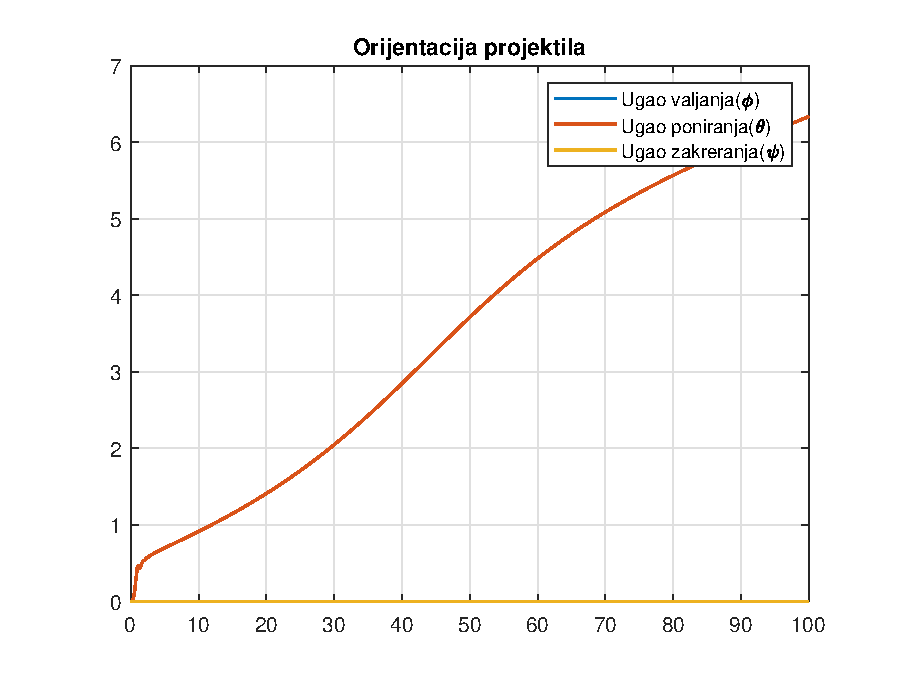
\includegraphics[scale = 0.5]{pitchVis.eps}
    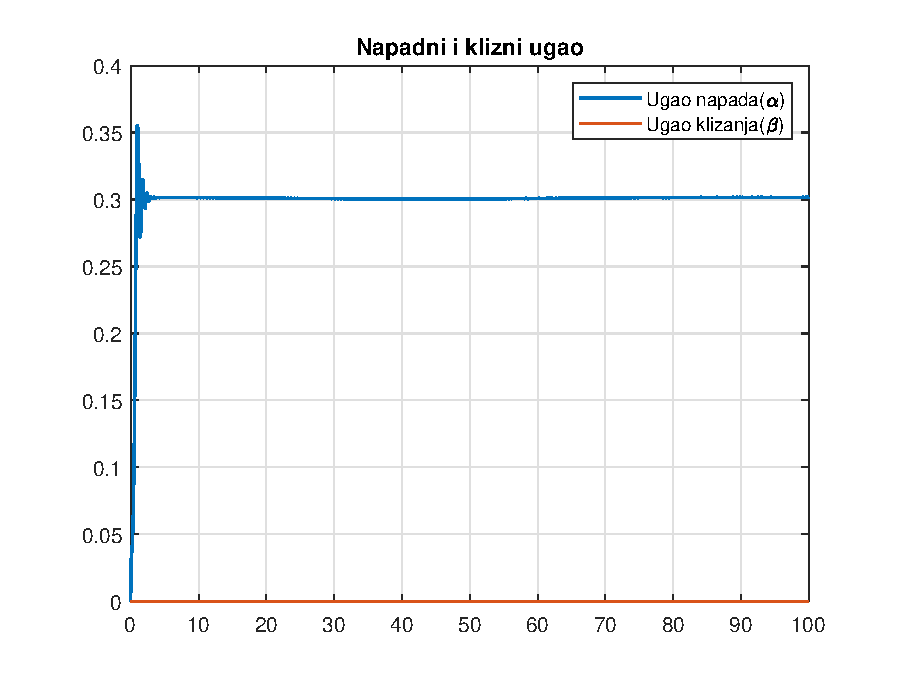
\includegraphics[scale = 0.5]{AoAvis.eps}
    \caption{Orijentacija projektila i ugao napada i klizanja pri jediničnom otklonu krmila 
    visine}
\end{figure}
Sada se vide očekivani rezultati. Kada se otkloni krmilo visine, projektil se usmjeri lagano prema gore. 
Grafik na kojem je prikazan ugao propinjnanja je dat u radijanima, pa se prema skoro linearnom 
odzivu može naslutiti da je putanja projektila kružne prirode. U ovu tvrdnju ćemo se uvjeriti poslije. Dalje,
vidimo da je napadni ugao konstantan u toku cijele putanje, što znači da se projektil uvijek kreće u smjeru $z$ ose tijela.
Ovo ne znači nužno da se projektil penje. Dalje, ugao klizanja je nula toko cijele putanje što 
znači da projektil ne skreće sa putanje, tj. da je vrijednost pomjeraja po $y$ osi uvijek nula. To se također 
vidi na graficima za ugao zakretanja. Treba primjetiti da je ugao valjanja također nula za jedinični otklon 
krmila visine. Ovo su itekako važni zaključci, jer se primjećuje da otklon krmila visine uzrokuje 
kretanje samo u vertikalnoj ravni pa se već naslućuje da postoji nezavisnost kretanja u vertikalnoj i horiznotalnoj 
ravni. Poslije ćemo se uvjeriti da je ova osobina od krucijalne važnosti za dizajn autopilota za zadatak vođenja. 
Sada pogledajmo, odzive brzina projektila koji su prikazani na slici \ref{fig:brzine}.
\begin{figure}[!ht]
    \centering 
    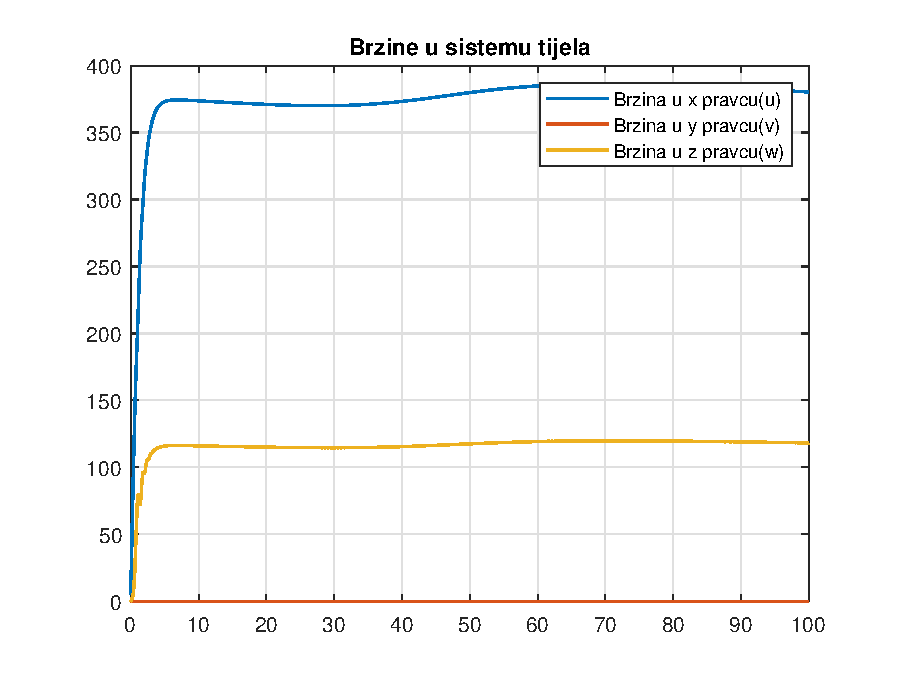
\includegraphics[scale =.5]{VbodyVis.eps}
    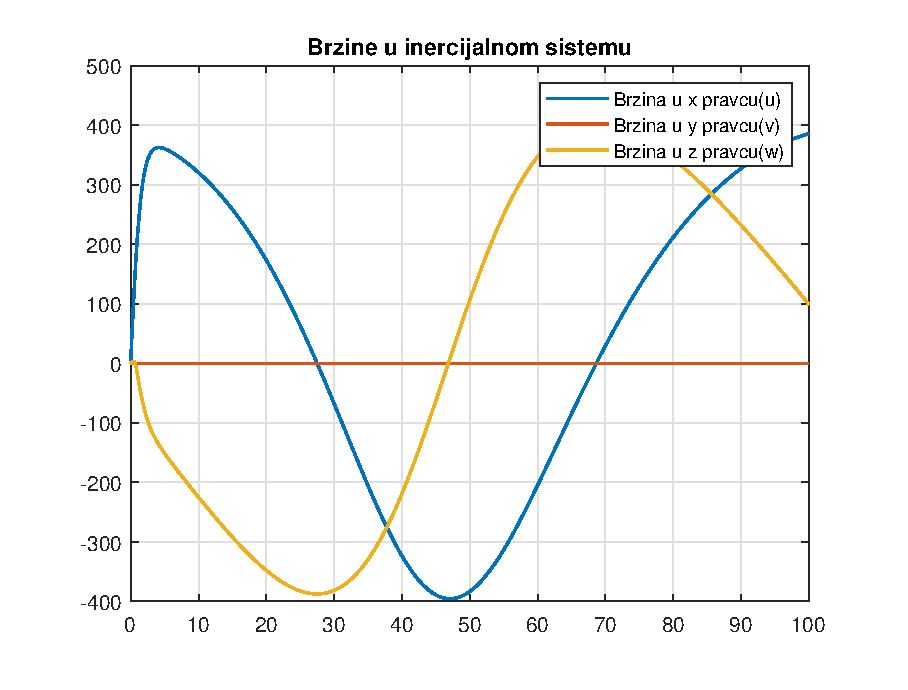
\includegraphics[scale =.5]{VinVis.eps}
    \caption{Brzine projektila u sistemu tijea i inercijalnom sistemu}
    \label{fig:brzine}
\end{figure}
Prvo što se primjeti jest da je brzina u $y$ smjerovima oba sistema uvijek nula. Dalje, posmatrajući 
sistem tijela vidi se da brzine nakon nekog vremena dostignu maksimalnu brzinu. Posmatrajući
sistema tijela, brzina u $x$ smjeru je stalna kao posljedica čeone sile otpora vazduha. Posmatrajući
inercijalni sistem, vidi se brzine u $x$ i $z$ smjeru imaju promjene koje sliče na kružno kretanje. Suma njihovih kvadrata 
će dati približno neku konstantnu vrijednost, pa se zaključuje da se projektil za slučaj otklona krmila visine, 
doista kreće po kružnici. Uvjerimo se u tu tvrdnju skicirajući putnaju projektila. Čitalac treba 
da primjeti da je na ovoj slici izvršena promjena znaka visine projektila. 
\begin{figure}[!ht]
    \centering 
    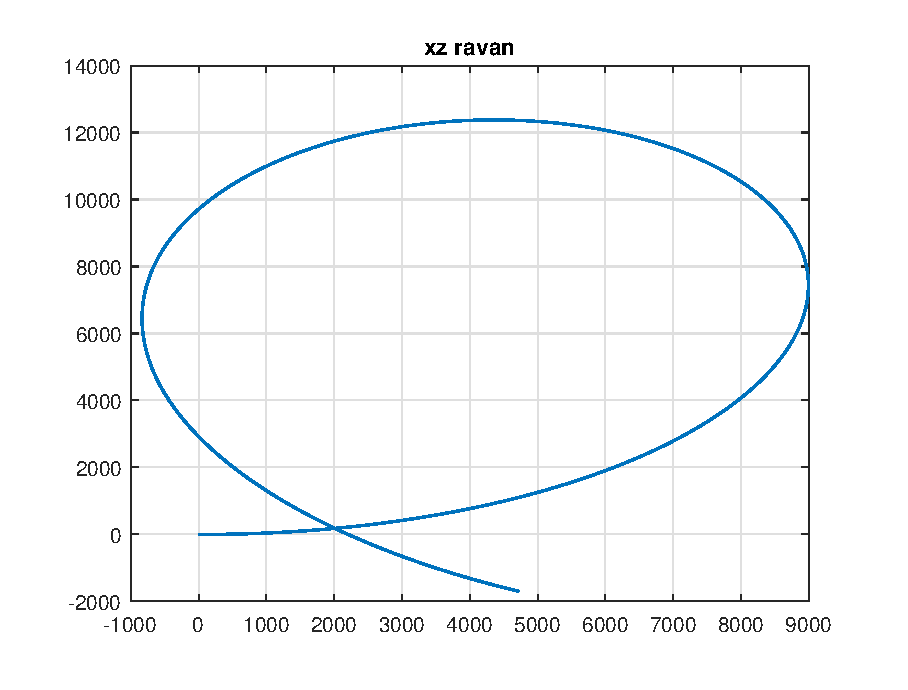
\includegraphics[scale= 0.5]{putnja2Dvis.eps}
    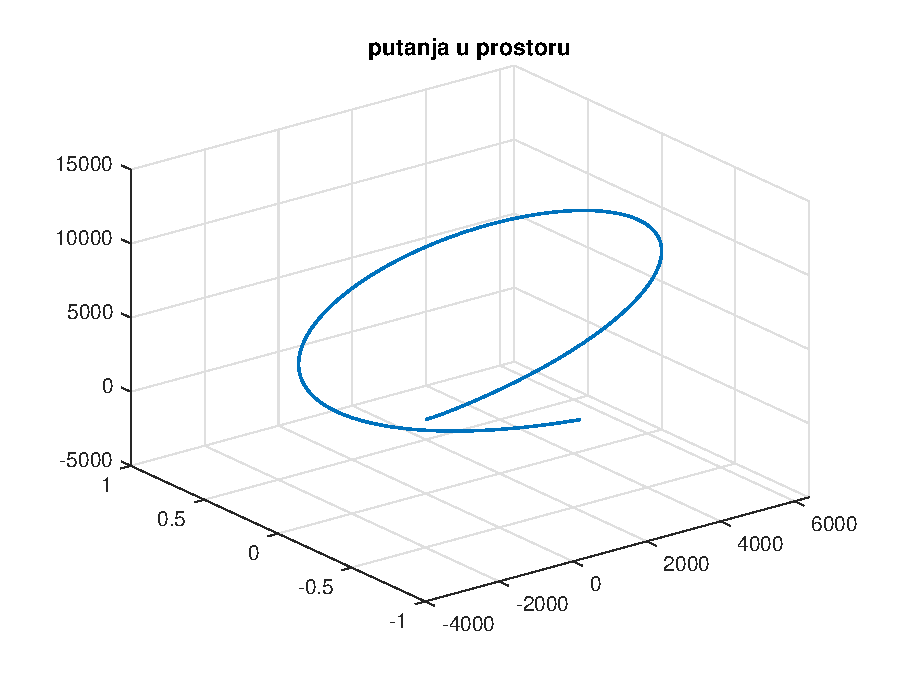
\includegraphics[scale= 0.5]{3dputanjaVis.eps}
    \caption{Putanja projektila za jedinični otklon krmila visine}
    \label{fig:2dpath}
\end{figure}
Sada se jasno vidi da projektil pravi kružnu putanju u prostoru. 
Poslije će se vidjeti da su normalna ubrzanje važna za proces vođenja projektila, pa treba razmotriti 
šta se dešava sa ubrzanjima kada se imaju otkloni kontrolnih površina. Na slici \ref{fig:ubrVis} su 
prikzani vertikalno i horizontalno ubrzanje projektila.
\begin{figure}[!ht]
    \centering 
    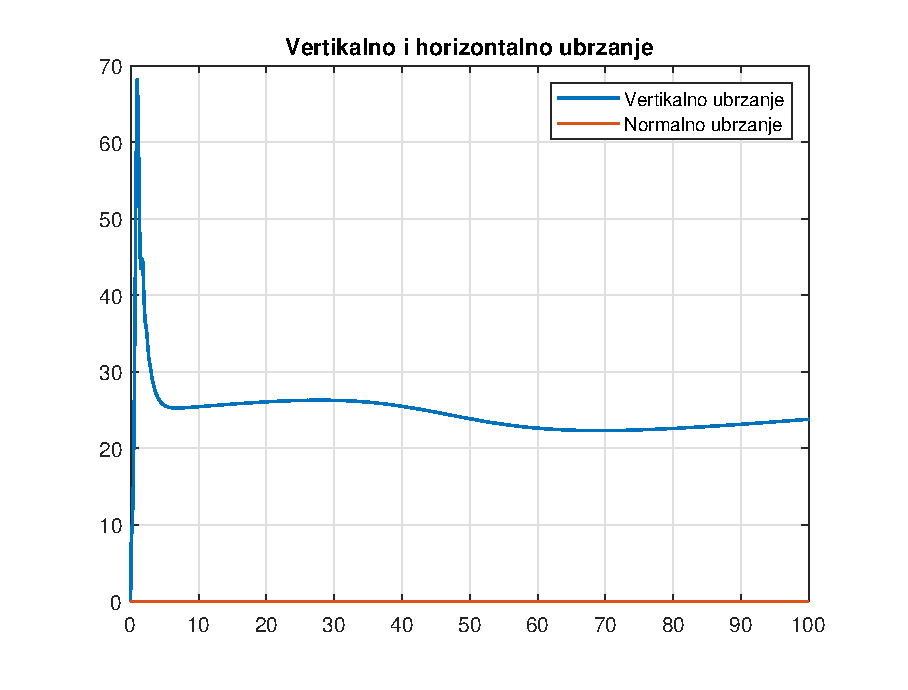
\includegraphics[scale= 0.5]{ubrVis.eps}
    \caption{Vertikalno i normalno ubrzanje projektila za jedinični otklon krmila visine}
    \label{fig:ubrVis}
\end{figure}
Sada se jasno vidi da se za jedinični otklon krmila visine postiže stalno vertikalno ubrzanje, što se slaže sa 
činjenicom da projektil čini kružnu putanju u $xz$ ravnini. Nulto horizontalno ubrzanje 
se slaže sa činjenicom da projektil ne čini pomjeraje u horiznotalnoj ravnini. 
Sada posmatrajmo odziv projektila za jedinični otklon krmila pravca. Ovdje će se izvršiti 
duža simulacija kako bi se dobila bolja analiza. Na slici \ref{fig:putanjePrav} su prikazane 
putanje u $xz$ i $xy$ ravninama kada se ima jedinični otklon krmila pravca projektila. 
\begin{figure}[!ht]
    \centering
    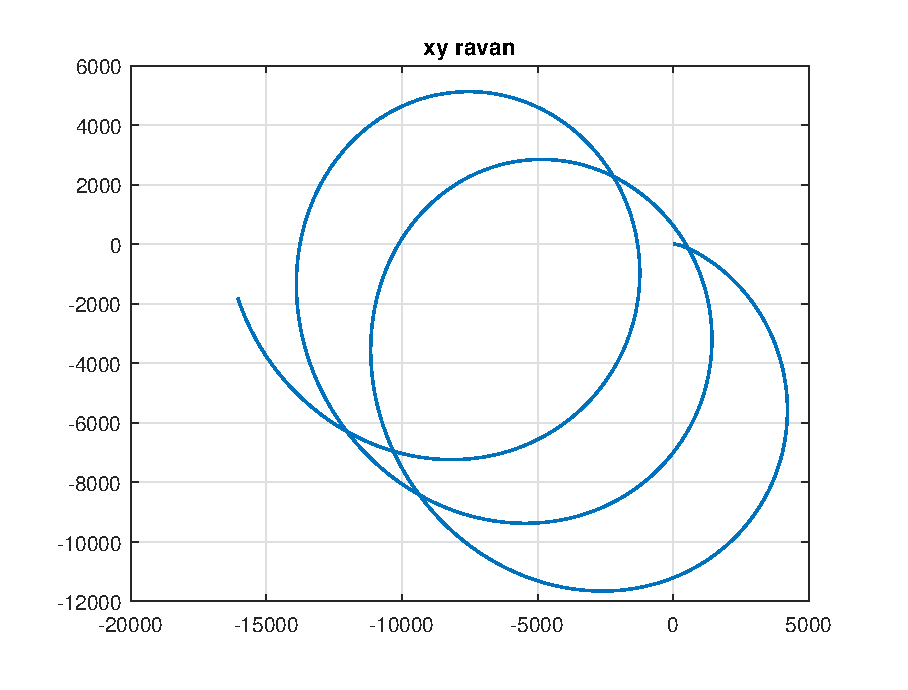
\includegraphics[scale=0.5]{xyPrav.eps}
    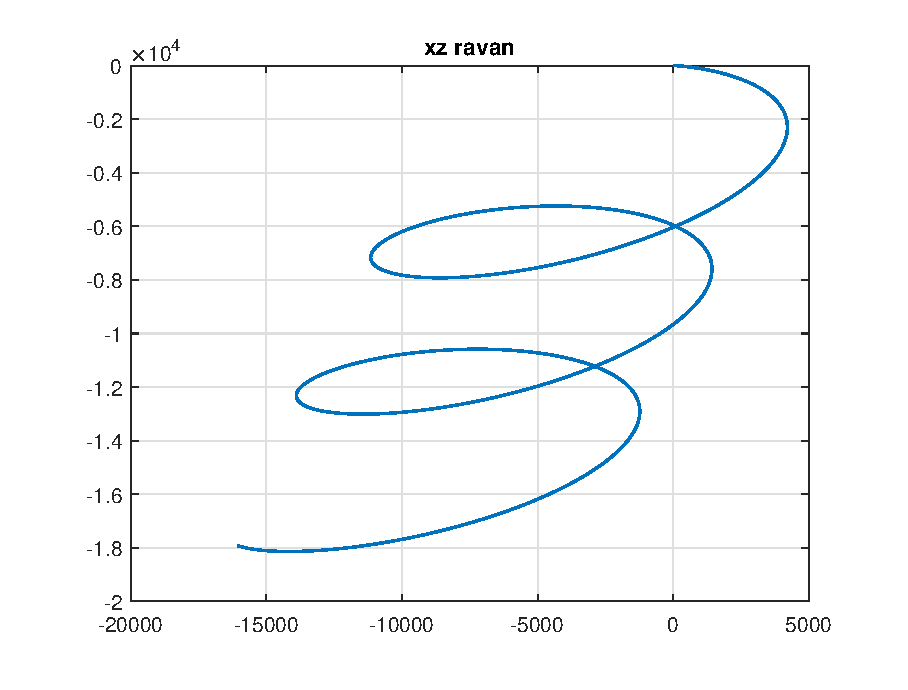
\includegraphics[scale=0.5]{xzPrav.eps}
    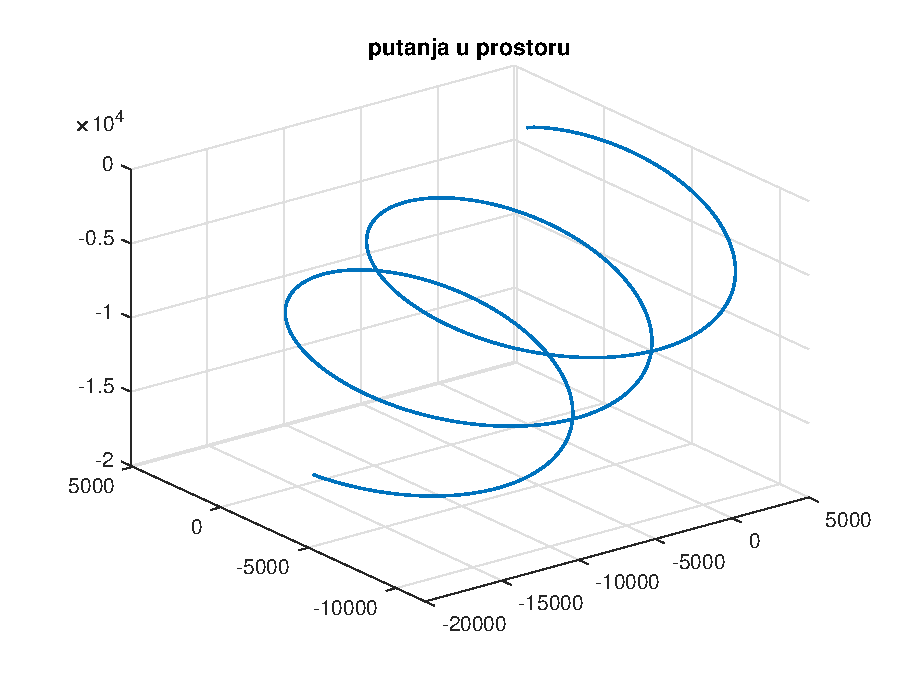
\includegraphics[scale=0.5]{3dprav.eps}
    \caption{Putanje pri jediničnom otklonu krmila pravca}
    \label{fig:putanjePrav}
\end{figure}
Sada se vidi da kada se zakrene krmilo visine, da projektil čini kružnu putanju u $xy$ ravni, što je bilo 
i očekivano. Naravno pomjeraj po $x$ osi mora da postoji zbog stalne sile potiska. Vidi se da u 
$xz$ ravnini, projektil pada na zemlju ali i treba primjetiti da se projektil u nekim 
trenucima počinje dizati po $z$ osi. Ovo je posljedica postojanja pogonske sile i statičke stabilnosti projektila. 
Pošto je centar gravitacije projektila ispred centra pritiska, projektil se počne rotirati tako da mu nos 
pokazuje ka zemlji, međutim zbog otklona krmila visine on počne rotirati u oko svoje $z$ ose pa u jednom trenutku 
njegov nos bude okrenut suprotno od zemlje te zbog pogonske sile kratko započne kretanje ka gore sve dok se 
zbog otklona krmila pravca ne nastavi rotirati i posljedično nastavi smanjivati visinu. 
Promjene orijentacije projektila se vide na slici \ref{fig:eulerPravac}
\begin{figure}[!ht]
    \centering
    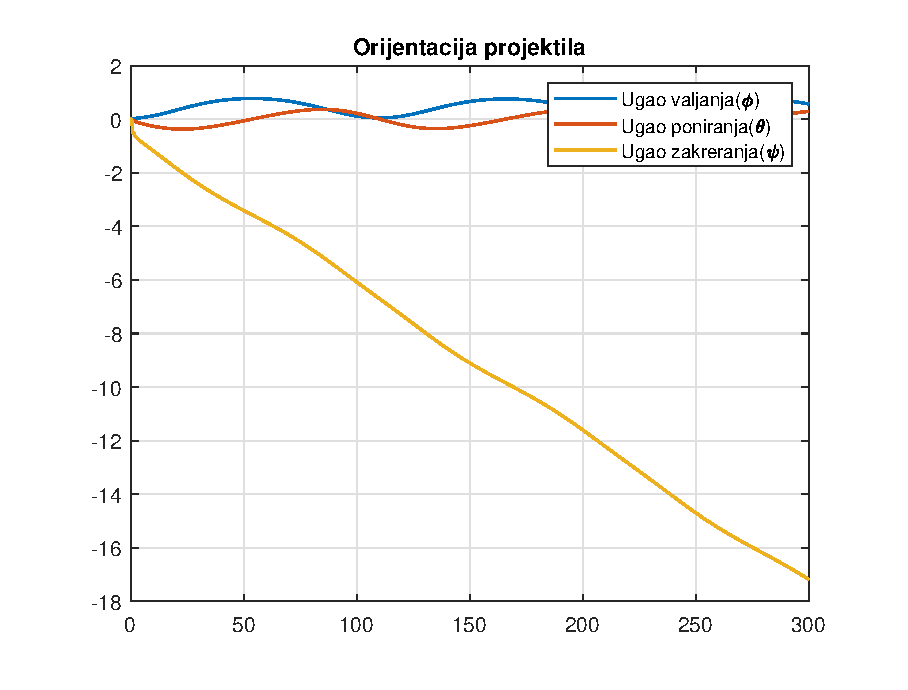
\includegraphics[scale = 0.5]{eulerPravac.eps}
    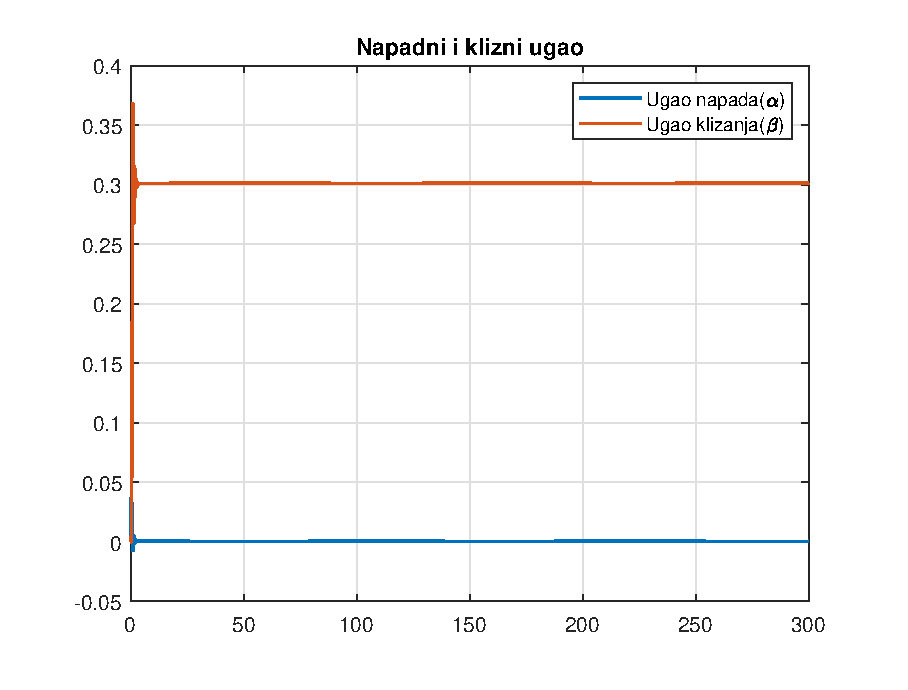
\includegraphics[scale = 0.5]{AOApravac.eps}
    \caption{Orijentacija projektila i ugao klizanja za jedinični otklon krmila pravca}
    \label{fig:eulerPravac}
\end{figure}
Vidi se na prethodnoj slici da ugao valjanja i ugao poniranja variraju, što objašnjava 
varijacije visine projektila i vidi se ugao zakretanja opada što objašnjava kružno kretanje 
u $xy$ ravnini. Posljedica toga je i konstantan ugao klizanja. Važno je istaći da je kanal pravca 
sistem neminimalne faze jer se za pozitivan otklon krmila pravca, dobija negativan odziv ugla zakretanja. 
U nastavku se posmatra primjer horizontalnog hitca početnom brzinom od $100m/s$ u $x$ smjeru
sa visine $500m$. Kada ne bi bilo otpora vazduha i pogonske sile za očekivati je da će projektiil pasti na zemlju 
za $10.09$ sekundi. Naravno, zbog postojanja pogonske sile projektil će za nešto kraće vrijeme 
dotaknuti tlo. Pri ovoj simulaciji pretpostavljen je jedinični otkolon elerona, pa će se pojaviti i valjanje. 
Na slici \ref{fig:eleronPutanja} su prikazane putanje kod ovog primjera. 
\begin{figure}[!ht]
    \centering
    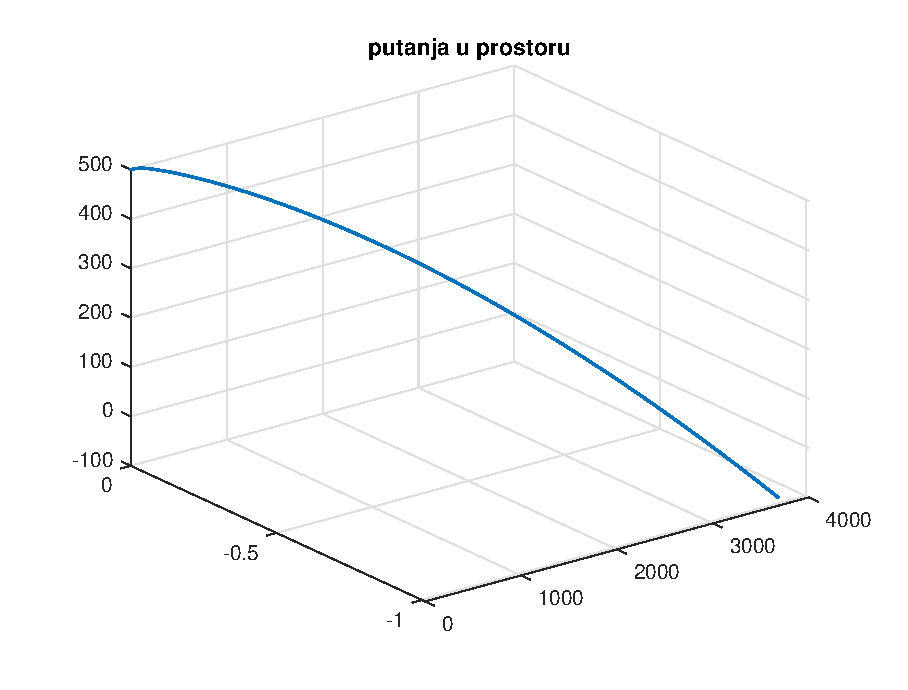
\includegraphics[scale = 0.7]{3deelron.eps}
    \caption{Trajektoija horizontalnog hitca sa jediničnim otklonom elerona}
    \label{fig:eleronPutanja}
\end{figure}
Vidi se da u ovom primjeru projektil, kao što je i očekivano, približno prati parabolu. 
Sada pogledajmo šta se dešava sa orijentacijom projektila. Na slici \ref{fig:orijentacijaEleron}
su prikazani Eulerovi uglovi. 
\begin{figure}[!ht]
    \centering
    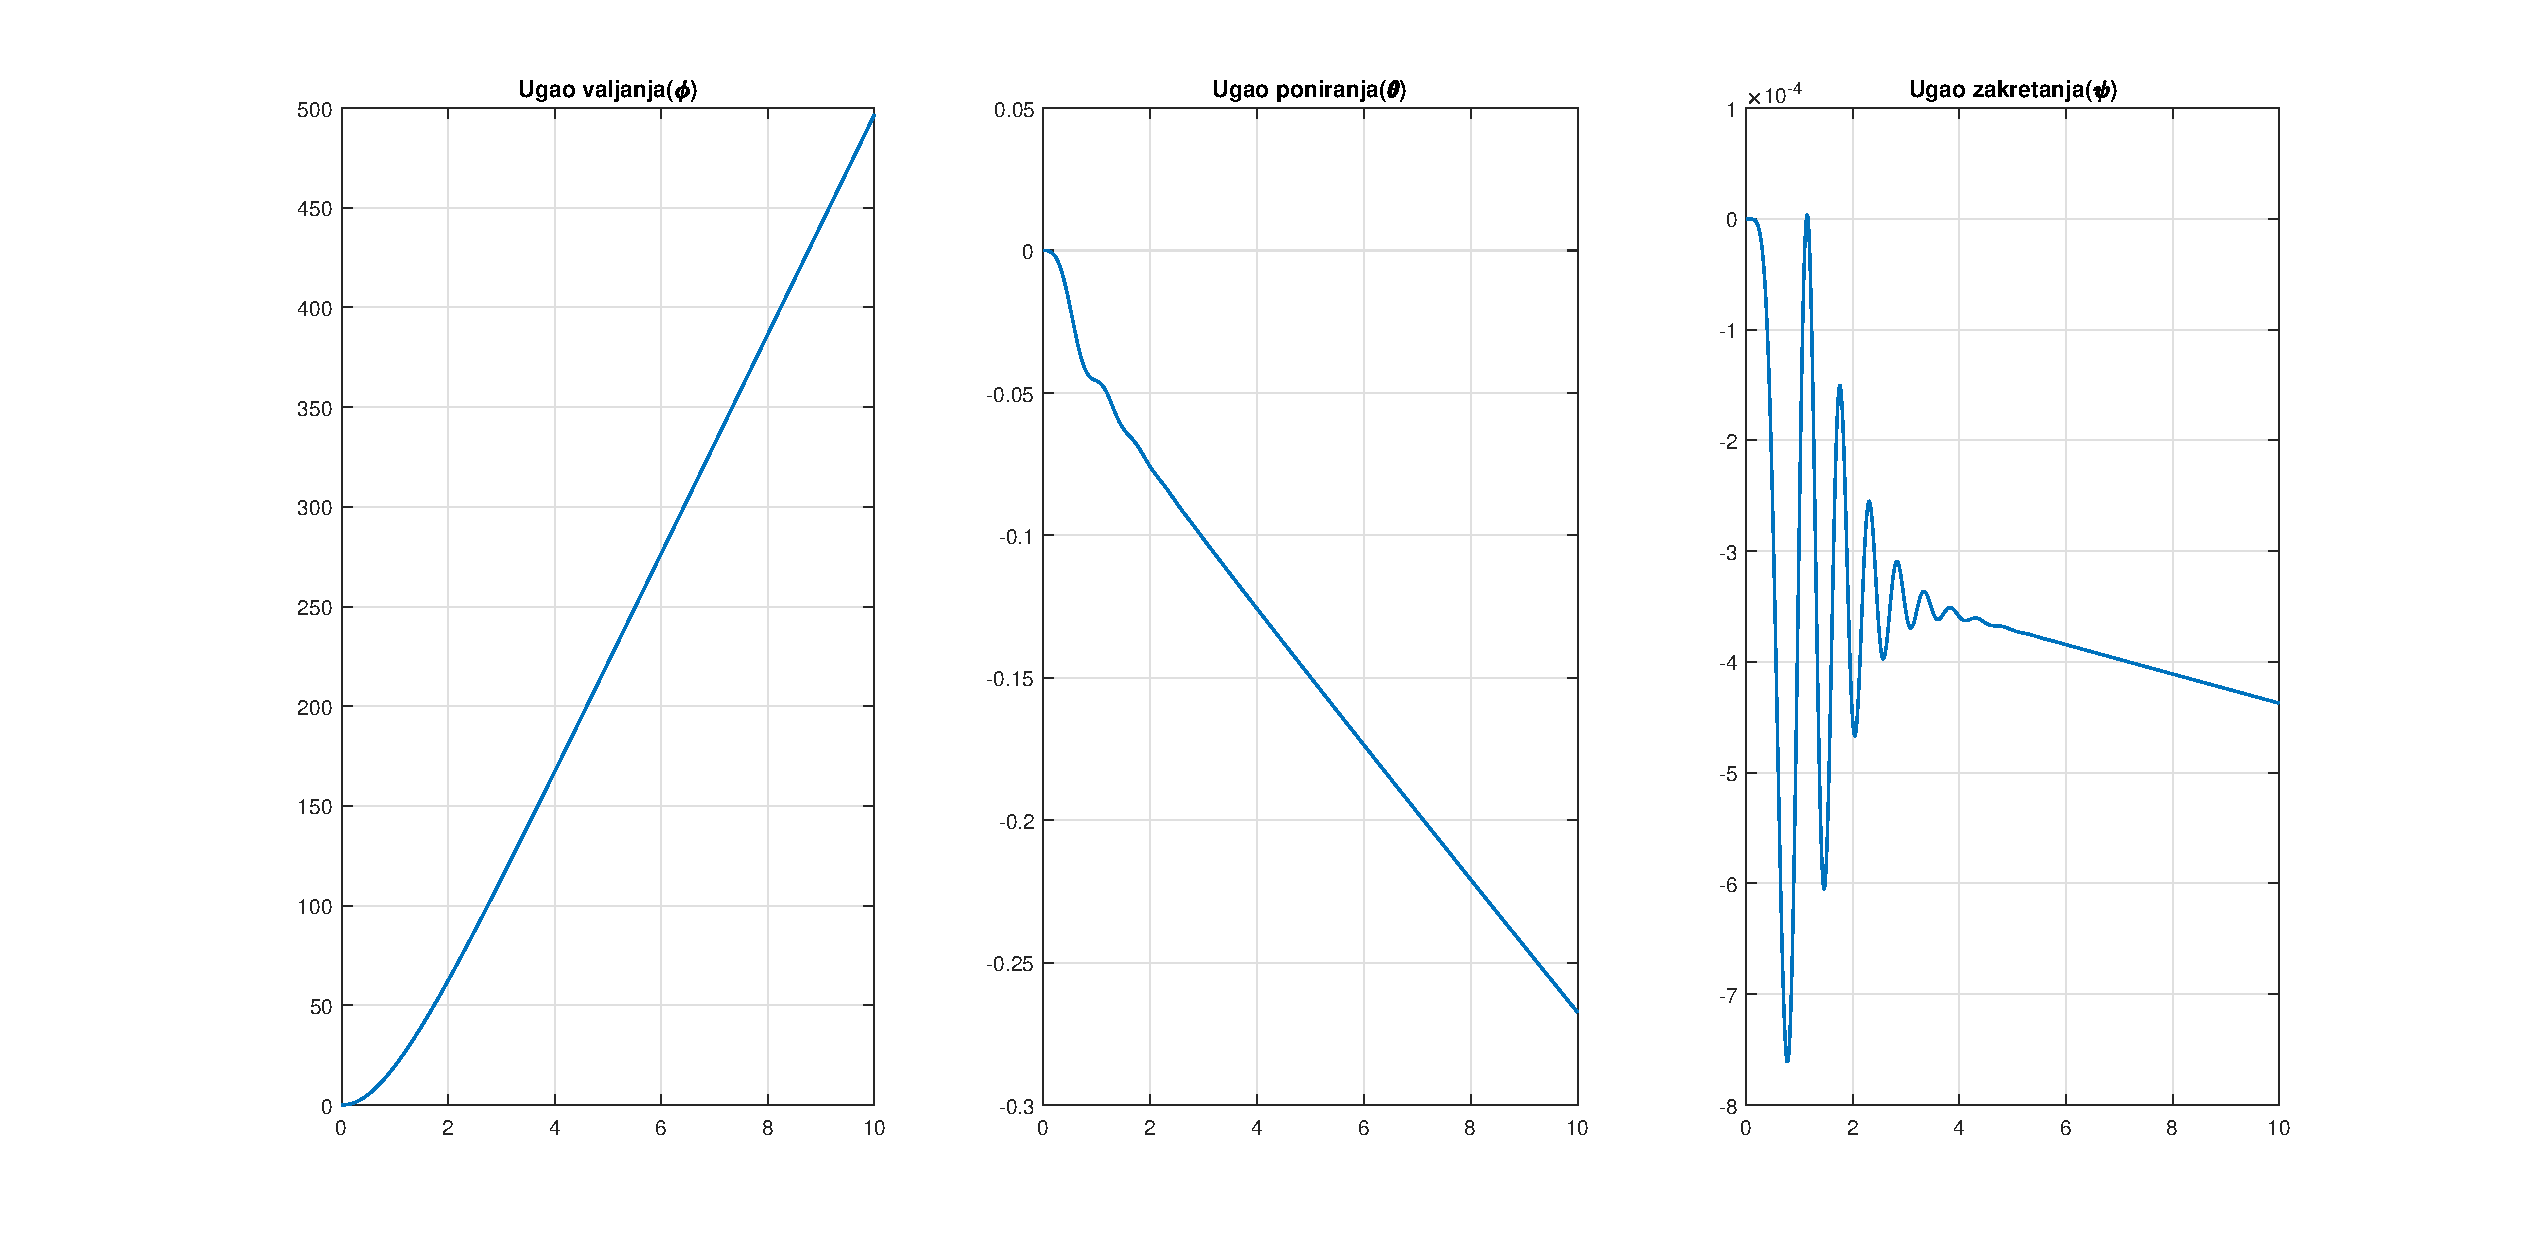
\includegraphics[scale = 0.4]{horHitacUglovi.eps}
    \caption{Orijentacija projektila pri horizontalnom hitcu sa jediničnim otklonom elerona}
    \label{fig:orijentacijaEleron}
\end{figure}
Zbog otklona elerona dolazi do porasta ugaone brzine valjanja što ima za posljedicu 
rast ugla valjanja. Prisjetimo se da se ugao valjanja ponaša kao čisti integrator i da je 
opisan diferencijalnom jednačinom:
\begin{equation*}
    \frac{dP}{dt} = L
\end{equation*}
Zbog ovoga za bilo kakvu promjenu otklona elerona, dolazi do rasta(po amplitudi) ugla valjanja. 
Promjena ugla propinjanja se može jednostavno objasniti pojavom uzgona. Pošto se centar pritiska nalazi 
iza centra gravitacije, javlja se moment koji zakreće projektil nadole. Kada bi simulacija duže trajala 
ugao propinjanja bi dosegao vrijednost skoro -90 stepeni. Posmatrajući treći grafik na kojem 
je prikazan ugao zakretanja vide se male promjene ugla zakretanaja(reda $10^{-4}$). U ovom primjeru,
bočno kretanje je zanemarljivo, ali ako postoje komponente brzine u sva tri smjera sistema tijela tada 
promjena brzine valjanja može imati ozbiljne posljedice na stabilnost projektila i čak dovodi u pitnaje proces vođenja.
Za bolji uvid, na slici \ref{fig:eleronUbrzanja} su prikazani vertikalno i horizontalno ubrzanje projektila(poslije će se pokazati 
da su vertikalno i horizontalno ubrzanje presudni za proces vođenja).  
\begin{figure}[!ht]
    \centering
    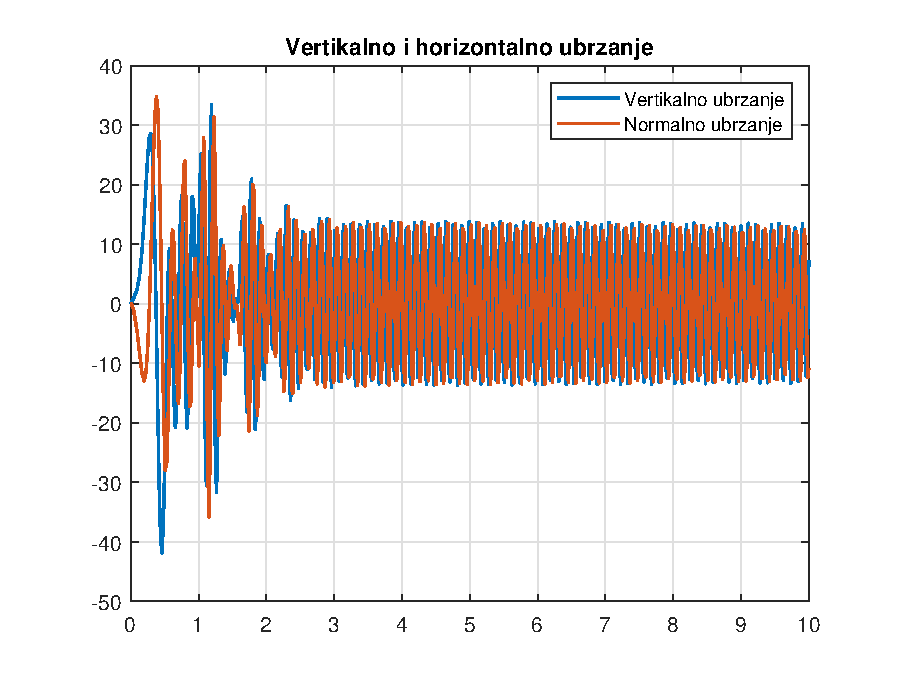
\includegraphics[scale=0.7]{eleronUbrzanja.eps}
    \caption{Vertikalno i normalno ubrzanje pri jediničnom otklonu elerona}
    \label{fig:eleronUbrzanja}
\end{figure}
Ovdje se vide velike oscilacije ubrzanja kada se pojavi kretanje u kanalu valjanja. Pošto se 
ova ubrzanja koriste kao referentna vrijednost kod vođenja projektila, neophodno je stabilizirati 
kanal valjanja kako bi se poboljšala regulacija ubrzanja. 
Dalje, pri velikim brzinama projektila i kretanju u kanalu valjanja dolazi do pojave couplinga 
kanala visine i kanala skretanja. Prema tome svi projektili krstaste konfiguracije 
kao prvi zahtjev pri dizajnu autopilota imaju stabilazaciju ugla valjanja. 
\section{Rasprezanje dinamičkog modela}
Sada će se u svrhu lakše analize i sinteze regulatora izvršiti rasprezanje dinamičkog modela. Ideja je 
da se uvedu neke pretpostavke koje će omogućiti da se predstavljene jednačine razdvoje na grupe 
nezavisnih jednačina.Treba da je ispunjeno:
\begin{itemize}
    \item Projektil se kreće u vertikalnoj ravni referentnog koordinatnog sistema.
    \item Osa $x_z$ leži u ravni kretnja.
\end{itemize}
Prva pretpostavka iziskuje $\beta , \phi , P, R\approx 0$. Činjenica da je $P,R \approx 0$ znači da se tijelo rotira samo oko $Y_b$ ose
,dalje, pretpostavka da je $\beta \approx 0$ znači da je usmjerenje letjelica isto kao i vektor brzine i konačno činjenica 
da je $\phi \approx 0$ znači da nema valjanja.  
Druga pretpostavka iziskuje $\Psi, \psi, y_z\approx 0$. Ovo znači da nema skretanja, da projektil može mjenjati samo visinu i udaljenost po $X_z$ osi.
Dakle ove dvije pretpostavke ograničavaju kretanje letjelice na vertikalnu ravan sa dopuštenjem propinjanja i kretanjem naprijed. 
Sada preostale jednačine koje su okarakterisane varijablama stanja:
\[V,\Theta,\theta,\alpha,Q,x_z, z_z\]
Definišu \textit{longitudinalno kretanje(kretanje u vertikalnoj ravni)}. Jednačine okarakterisan varijablama 
koje su u ovom slučaju zanemarene definišu \textit{lateralno kreetanje(bočno)} koje se sastoji 
od kretanja u horizntalnoj ravni, skretanja i valjanja ali bez propinjanja. Sada se ova dva podsistema mogu odvojeno posmatrati.
Sada ostaje samo da se sile koje su objašnjenje u prethodnom poglavlju pretvorimo iz sistema tijela 
i sistema Zemlje u sistem brzine i da ih se uvrsti u jednačine koje opisuju model u sistemu brzine. 
Jednačine koje predstavljaju longitudinalno kretanje su:
\begin{align}
    &m\frac{dV}{dt}= P\cos\alpha - R_{otp} - G\sin\Theta\\
    &mV\frac{d\Theta}{dt} = -Psin\alpha - R_{uzg} + G\cos\Theta\\
    &I_x\frac{dQ}{dt} \approx M\\
    &\frac{d\theta}{dt}=Q\\
    &\frac{dx_z}{dt}=V\cos\Theta\\
    &\frac{dz_z}{dt}=-V\sin\Theta
\end{align}
Također iz matrice transformacije $Tz^v$(treba invertovati $Tv^z$) se dobija za uvedene pretpostavke:
\begin{equation}
    \Theta = \theta - \alpha
\end{equation}
Sada se mogu napisati i jednačine za lateralno kretanje:
\begin{align}
    &mVcos\Theta \frac{d\Psi}{dt}=-P\cos\alpha \sin\beta \cos\phi - P\sin\alpha\sin\phi 
    - R_{side}\cos\phi - R_{uzg}\sin\phi\\
    &I_x\frac{dP}{dt}=L\\
    &I_z\frac{dR}{dt}=N+(I_x-I_y)\\
    &\frac{d\psi}{dt}=(R\cos\phi+q\sin\phi)/\cos\theta\\
    &\frac{d\theta}{dt}=P+(R\cos\phi - q\sin\phi)/\tan\theta\\
    &\frac{dy_z}{dt}=V\cos\Theta\sin\Psi
\end{align}
Pri čemu se iz $Tz^v$ pokazuje:
\begin{equation}
    \Psi \approx \psi-\beta
\end{equation}
Još uvijek se nisu u diferencijalne jednačine uvele linearizirane vrijednosti za aerodinamičke 
sile i momente pa se u jednačinama ne pojavljuju upravljačke varijable, zbog toga će se u nastavku uraditi
poptuna linearizacija dinamičkog modela. Tada će se dobiti zavisnost varijabli stanja od ulaza, pa 
je na osnovu toga moguće riješiti ove jednačine da bi se odredile varijable stanja. Iz ovoga slijedi i obrat 
tj. da se mogu odrediti otkloni upravljačkih površina da bi se postigle željene vrijednosti varijabli stanja 
koje zahtjeva zakon voođenja. Naravno ovakav postupak je u otvorenoj petlji pa se zbog netačnosti modela 
preporučuje upravljanje u zatvorenoj povratnoj sprezi. 
\section{Linearizacija u okolini nominalne trajektorije}
Generalno, kada se priča o linearizaciji sistema, radi se o linearizaciji oko neke radne tačke. Ideja je 
da se diferencijalna jednačina u okolini te radne tačke predstavi linearnim segmentnom, te da 
nakon toga ona ima linearnu zavisnot od ulaznih parametara. Kod kretanja projektila umjesto pojma 
radne tačke se uvodi pojam \textit{nominalne trajektorije}. To je trajektorija po kojoj projektil 
leti kada su sve varijable stanja upravo onakve kako se od njih očekuje da budu i kada nema vanjskih poremećaja 
na projektil osim aerodinamičkog otpora i gravitacije. Sada se kao suprotnost nominalnoj trajektoriji 
uvodi pojam \textit{poremećajnog kretanja} koje se odlikuje odstupanjem varijabli stanja od nominalnih vrijednosti. 
Pri ovome se pretpostavlja da su odstupanja varijabli stanja pri poremećajnom kretanju relativno mala u odnosu na 
njihove nominalne vrijednosti. Svaka nominalna trajektorija određena je nekom vrijednošću vektora stanja $X_{nom}$.
Do ostalih vrijednosti može se doći rješavanjem jednačine:
\begin{equation}
    \dot{\vec{X}}_{nom} = f(\vec{X}_{nom}, \delta_{nom})
\end{equation}
Sada će se izvšiti linearizacija modela longitudinalnog kretanja. Pretpostavlja se da u okolini radne tačke, 
vrijednosti varijabli stanja imaju oblik:
\begin{equation}
    x=x_0+\Delta x 
\end{equation}
Prisjetimo se samo da u okolini nominalne trajektorije upravljački signal može definisati kao:
\begin{equation}
    u(t) = u_0(t)+\Delta u(t)
\end{equation}
Pa je:
\begin{equation}
    \dot{x}_0(t)+\Delta \dot{x}(t)=f(x_0(t)+\Delta x(t),u_0(t)+\Delta u(t))
\end{equation}
Funkcija na desnoj strani se može raziti u Taylorov red i nakon odbacivanja članova višeg reda
se dobija:
\begin{equation}
    \dot{x}_0(t)+\Delta \dot{x}(t)=f(x_0(t),u_0(t))+\frac{\partial f}{\partial x}\Delta x+\frac{\partial f}{\partial u}\Delta u
\end{equation}
Sada se može napisati:
\begin{equation}
    \Delta \dot{x}(t)=\frac{\partial f}{\partial x}\Delta x+\frac{\partial f}{\partial u}\Delta u
\end{equation}
Parcijalni izvodi se uzimaju tako da vrijedi $x=x_0$ i $u=u_0$.\\
Kod modela longitudinalnog kretanja će se izvršiti isti postupak s tim da će se linearizirati svaka 
jednačina posebno. Sada za model longitudinalnog kretanja, ako se pretpostavi da se 
projektil kreće po nominalnoj trajektoriji, vrijede jednačine:
\begin{align}
    &V=V_0+\Delta V \\
    & \alpha = \alpha _0+\Delta \alpha\\
    & \Theta=\Theta _0 +\Delta \Theta\\
    & \theta= \theta _0+\Delta \theta\\
    & Q=Q_0+\Delta Q\\
    & z_z=z_{z0}+\Delta z_z\\
    & \delta _V=\delta _{V0}+\Delta \delta _V
\end{align}
Koristeći pretpostavku da je $\cos\alpha_0 \approx 1$ i koristeći gore predstavljenu metodologiju 
linearizacije može se dobiti:
\begin{align}
    &\frac{d\Delta V}{dt}=\frac{P^V-F_o^V}{m}\Delta V - \frac{P\alpha+F_0^\alpha}{m}\Delta\alpha - g\cos\Theta _0\Delta\Theta +\frac{F_u^{\delta )V}}{m}\delta_V+\frac{X_P}{m}\\
    &\frac{d\Delta \Theta}{dt}=\frac{P^V-F_u^V}{m}\Delta V + \frac{P-F_u^\alpha}{mV}\Delta \alpha-\frac{g}{V}\sin\Theta\Delta\Theta-\frac{F_u^{\delta_V}}{\Delta_V}+\frac{Z_P}{mV}\\
    &\frac{d\Delta Q}{dt}=\frac{M^V}{I_y}\Delta V+\frac{M^\alpha}{I_y}\Delta Q+\frac{M^{\dot{\alpha}}}{I_y}\Delta\dot{\alpha}+\frac{M^{\delta_V}}{I_y}\Delta \delta_V+\frac{M^{\dot{\delta}_V}}{I_y}\Delta \dot{\delta}_V+\frac{M_P}{I_y} \\
    &\frac{d\Delta \theta}{dt}=\Delta Q \\
    &\frac{d\Delta x_z}{dt}=\cos\Theta_0\Delta V-V\sin\Theta_0\Delta\Theta\\
    &\frac{d\Delta z_z}{dt}=\sin\Theta_0\Delta V+V\cos\Theta_0\Delta\Theta \\
    &\Delta\alpha=\Delta\theta - \Delta\Theta
\end{align}
U koeficijentima dobijenih diferencijalnih jednačina su eksponentima označeni izvodi te veličine. Konkretno, 
$P^V=\frac{\partial P}{\partial V}$, $F_o^\alpha = \frac{\partial F_o}{\partial \alpha} = QSC_o^\alpha$ etc. 
Svi ovi parcijalni izvodi su objašnjeni kada se govorilo o prirodi aerodinamičkih sila i momenata i oni se često 
za projektil daju tabelarno. Članovi $X_P$, $Z_P$ i $M_P$ predstavljaju poremećaje u vidu sila i momenata i oni ovdje 
djelom predstavljaju ulaze u sistem. Sada se u ovim jednačinama po prvi put eksplicitno vide upravljačke varijable.  
Na isti način se mogu naći i lineariziane jednačine za lateralno kretanje.
Ako se nađe Laplasova transformacija gornjih jednačina, rješavanjem dobijenog sistema algebarskih jednačina 
dobija se karakteristični polinom funkcija prenosa(sjetimo se da kod MIMO sistema, sve prenosne funkcije imaju isti karakteristični polinom). 
Radi se o polinomu četvrtog reda kod kojeg je jedan par polova po modulu dosta veći od drugog para polova po modulu. 
Sada je jasno da se kretanje letjelice može razdovjiti na \textit{brzo prigušeno} kretanje koje može biti oscilatorno 
ili aperiodičko i na \textit{fugoidno(sporo prigušeno)}. Dinamiku modela longitudinalnog kretanja određuje 
dominantni par polova koji je manji po modulu pa je kretanje letjelice određeno fugoidnim kretanje. Sada je jasno da se 
polovi koji opsiuju brzoprigušeno kretanje mogu odbaciti pa će karakteristčni polinom imati samo dva pola. 
Dakle, sada se posmatraju samo jednačine koje opisuju kratkoperiodično kretanje. Brzoperiodično kretanje je 
određeno jednačinom promjene brzine(prva diferencijalna jednačina) pa se nakon uvođenja ove pretpostavke odbacuje ova 
jednačina  i u ostalim se anulira $\Delta V$. Sada teba primjetiti da se u lineariziranim jednačinama pojavljuje koeficijent 
$-\frac{g}{V}\sin\Theta_0$. Ovaj koeficijent predstavlja uticaj gravitacije na longitudinalno kretanje. Za male elevacione 
uglove, ovaj koeficijent je jako blizak nuli. Čak i kada trajektorija puno odstupa od horizontalne, brzina projektila 
je najmanje 20 puta veća od gravitacionog ubrzanja pa se uticaj gravitacije na longitudinalno kretanje može zanemariti. 
Ova pretpostavka u prenosnim funkcijama uvodi pol u nuli, tj. pod ovom pretpostavkom sistem će se ponašati kao integrator i 
sam će osigurati nultu grešku stacionarnog stanja. Međutim ako ova pretpostavka nije ispunjenja tada će se pojaviti pol blizak nuli, 
pa će prelazni proces biti dug možda čak i nestabilan. Sada, pod ovim pretpostavkama dobijaju sljedeće prenosne funkcije:
\begin{align}
    &\frac{\Delta \theta(s)}{\Delta \delta_V(s)}=\frac{K(T_1s+1)}{s(T^2s^2+2\xi Ts+1)}\\
    &\frac{\Delta \Theta(s)}{\Delta \delta_V(s)}=\frac{K}{s(T^2s^2+2\xi Ts+1)}\\
    &\frac{\Delta \alpha(s)}{\Delta \delta_V(s)}=\frac{KT_1}{T^2s^2+2\xi Ts+1}\\
    &\frac{\Delta n_z(s)}{\Delta \delta_V(s)}=\frac{V}{g}\frac{K}{T^2s^2+2\xi Ts+1}
\end{align}
,gdje $n_z = \frac{V\dot{\Theta}}{g}$ predstavlja \textit{normalno preopterećenje}, tj. odnos ubrzanja koje je normalno na pravac brzine i gravitacione konstante. 
Normalno ubrzanje je definisano izrazom:
\begin{equation}
    a_z = V\dot{\Theta} + g\cos\Theta
\end{equation}
I predstavlja jako bitnu veličinu jer mnogi zakoni vođenja generišu komandne signale u vidu normalnog ubrzanja projektila, pa će se i 
posebna pažnja posvetiti upravljanju normalnog ubrzanja. Prenosna funkcija koja određuje normalno ubrzanje je:
\begin{equation}
    \frac{\Delta a_z(s)}{\Delta \delta_V(s)} =\frac{KV}{T^2s^2+2\xi Ts+1}
\end{equation}
\begin{figure}[!ht]
    \centering
    \begin{tikzpicture}[auto, node distance=2cm,>=latex']
        \node[input, name=input](input){};
        \node[block, right of = input, node distance = 3cm] (g1){$\frac{KT_1}{T^2s^2+2\xi Ts+1}$};
        \node[block, right of = g1, node distance = 3cm] (g2) {$\frac{T_1s+1}{T_1s}$};
        \node[block, right of = g2] (g3){$\frac{1}{1+T_1s}$};
        \node[anchor = south] (alpha) at ($(g1)!0.6!(g2)$){$\alpha$};
        \node[anchor = south] (theta) at ($(g2)!0.5!(g3)$){$\theta$};
        \node [output, right of = g3] (output) {};
        \node[block, below of = g3] (g4) {$\frac{V}{gT_1}$};
        \node [output, right of = g4] (output2) {};
        \draw [->] (g3) -- node [name=y] {$\Theta$}(output);
        \draw[->] (g4)--node[] {$n_z$}(output2);
        \draw[->] (alpha)|-(g4);
        \draw [draw,->] (input) -- node {$\delta_V$} (g1);
        \draw[->](g1)--(g2);
        \draw[->](g2)--(g3);
\end{tikzpicture}
\caption{Blok dijagram lineariziranog modela longitudinalnog kretanja}
\label{fig:diagLongi}
\end{figure}
Evidentno je da za dobijanje lineariziranog modela longitudinalnog kretanja uvedeno 
puno pretpostavki i da će bilo kakvo odstupanje od ovih pretpostavki umanjiti vjerodostojnost modela, 
ali se pokazuje da je ovaj linearizirani model dosta dobra aproksimacija pri nominalnim uslovima leta. 
